%---------------------------------------------------------------------------
% MBS Benchmark A04: Bricard's Mechanism
%---------------------------------------------------------------------------
%
% LaTeX Template: Jacobs Landscape Poster
% Created by:
% Computational Physics and Biophysics Group, Jacobs University
% https://teamwork.jacobs-university.de:8443/confluence/display/CoPandBiG/LaTeX+Poster



%----------------------------------------------------------------------------------------
%	PACKAGES AND OTHER DOCUMENT CONFIGURATIONS
%----------------------------------------------------------------------------------------

\documentclass[final]{beamer}

\usepackage[scale=1.24]{beamerposter} % Use the beamerposter package for laying out the poster

\usetheme{confposter} % Use the confposter theme supplied with this template

\setbeamercolor{block title}{fg=ngreen,bg=white} % Colors of the block titles
\setbeamercolor{block body}{fg=black,bg=white} % Colors of the body of blocks
\setbeamercolor{block alerted title}{fg=white,bg=dblue!70} % Colors of the highlighted block titles
\setbeamercolor{block alerted body}{fg=black,bg=dblue!10} % Colors of the body of highlighted blocks
% Many more colors are available for use in beamerthemeconfposter.sty

%-----------------------------------------------------------
% Define the column widths and overall poster size
% To set effective sepwid, onecolwid and twocolwid values, first choose how many columns you want and how much separation you want between columns
% In this template, the separation width chosen is 0.024 of the paper width and a 4-column layout
% onecolwid should therefore be (1-(# of columns+1)*sepwid)/# of columns e.g. (1-(4+1)*0.024)/4 = 0.22
% Set twocolwid to be (2*onecolwid)+sepwid = 0.464
% Set threecolwid to be (3*onecolwid)+2*sepwid = 0.708

\newlength{\sepwid}
\newlength{\onecolwid}
\newlength{\twocolwid}
\newlength{\threecolwid}
\setlength{\paperwidth}{48in} % A0 width: 46.8in
\setlength{\paperheight}{36in} % A0 height: 33.1in
\setlength{\sepwid}{0.024\paperwidth} % Separation width (white space) between columns
\setlength{\onecolwid}{0.301\paperwidth} % Width of one column
\setlength{\twocolwid}{0.602\paperwidth} % Width of two columns
\setlength{\threecolwid}{0.903\paperwidth} % Width of three columns
\setlength{\topmargin}{-0.5in} % Reduce the top margin size
%-----------------------------------------------------------

\usepackage{graphicx}  % Required for including images
\graphicspath{{../MBSfigures/}}
\usepackage{booktabs} % Top and bottom rules for tables

\usepackage{multirow}
\usepackage{siunitx}
%----------------------------------------------------------------------------------------
%	TITLE SECTION 
%----------------------------------------------------------------------------------------

\title{MBS Benchmark A04: Bricard's Mechanism} % Poster title




%----------------------------------------------------------------------------------------

\begin{document}

%\addtobeamertemplate{block end}{}{\vspace*{2ex}} % White space under blocks
%\addtobeamertemplate{block alerted end}{}{\vspace*{2ex}} % White space under highlighted (alert) blocks

\setlength{\belowcaptionskip}{2ex} % White space under figures
\setlength\belowdisplayshortskip{2ex} % White space under equations

\begin{frame}[t] % The whole poster is enclosed in one beamer frame

\begin{columns}[t] % The whole poster consists of three major columns, the second of which is split into two columns twice - the [t] option aligns each column's content to the top

\begin{column}{\sepwid}\end{column} % Empty spacer column

\begin{column}{\twocolwid} % The first column

%----------------------------------------------------------------------------------------
%	OBJECTIVES
%----------------------------------------------------------------------------------------

\begin{alertblock}{Benchmark Objective}
Bricard's mechanism (benchmark problem \textbf{A04})~\cite{bricard1897memorie} is an example of over-constrained system. 
Gr\"{u}bler's formula~\cite{grubler1884allgemeine} results in no degrees of freedom, however, the particular orientation of the revolute pairs results in a system with 1 degree of freedom.
\end{alertblock}



%----------------------------------------------------------------------------------------
%    BENCHMARK DESCRIPTION
%----------------------------------------------------------------------------------------





\begin{columns}[t, totalwidth=\twocolwid]

\begin{column}{0.95\onecolwid}
\begin{block}{Benchmark Description}
The system is composed of five rods and six revolute joints. Gravity is acting in the negative $y$ direction.

 Tab.~\ref{TAB:SystemProperties} reports system properties.


\end{block}


\begin{figure}
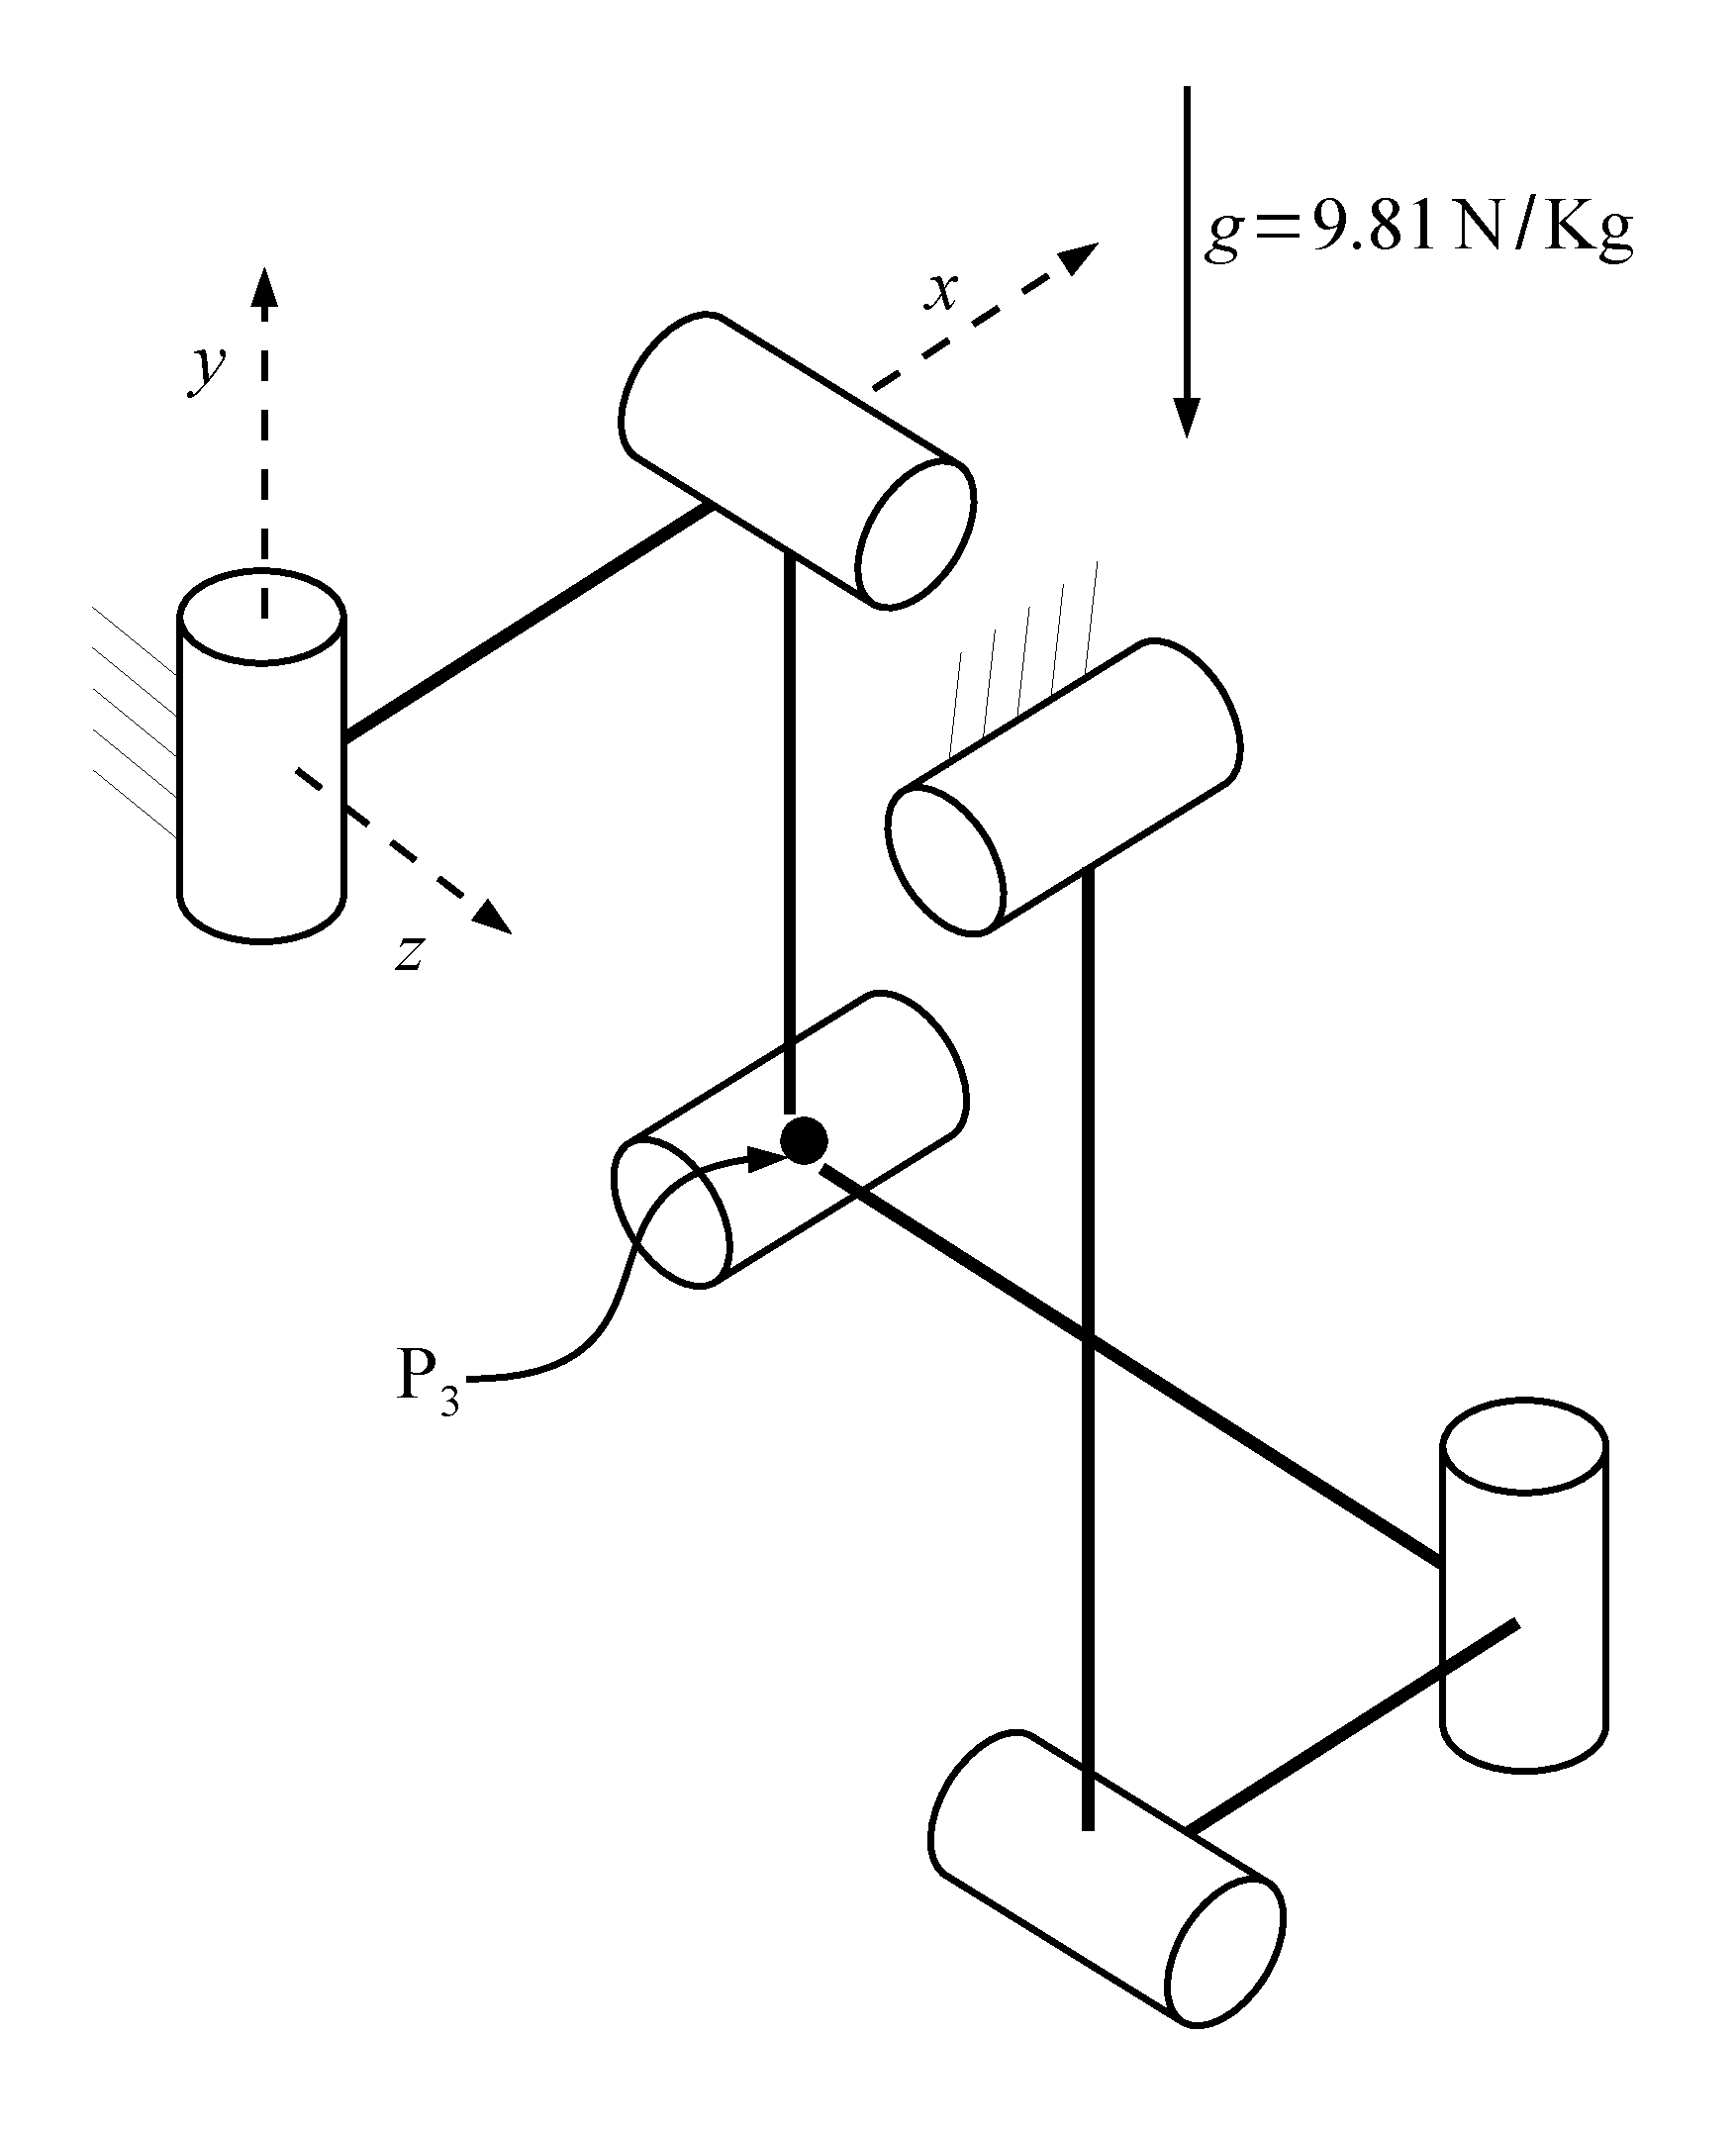
\includegraphics[width=0.8\linewidth]{4MBS_Bricard.pdf}
\caption{Bricard's mechanism sketch.}
\label{FIG:Bricard}
\end{figure}

\centering
\begin{table}
\begin{large}
	\begin{tabular}[b]{ll}
%\multicolumn{2}{c}{\textbf{System Properties}}\\
	\toprule
	Rods mass & $\SI{1.0}{\kilogram}$\\
	Rods length & $\SI{1.0}{\meter}$\\	
	\bottomrule
	\end{tabular}
	\end{large}
	\caption{System Properties and Configuration}
    \label{TAB:SystemProperties}
\end{table}
\end{column}

\begin{column}{0.95\onecolwid}



%----------------------------------------------------------------------------------------
%    RESULTS
%----------------------------------------------------------------------------------------



\begin{block}{Results}
The dynamic simulation of the \textbf{A04} benchmark was executed for \SI{600}{\second}. Fig.~\ref{FIG:Bricard} shows the Bricard's Mechanism in its initial position.
$P_3$ displacements estimated with the OpenSim simulation are compared with the values provided as reference~\cite{gonzalez2006benchmarking}.  

Fig.~\ref{FIG:simulationPlot} shows the outputs of OpenSim-based simulation and the benchmark references~\cite{gonzalez2006benchmarking} for a \SI{10}{\second} period.


\begin{figure}[h]
\centering
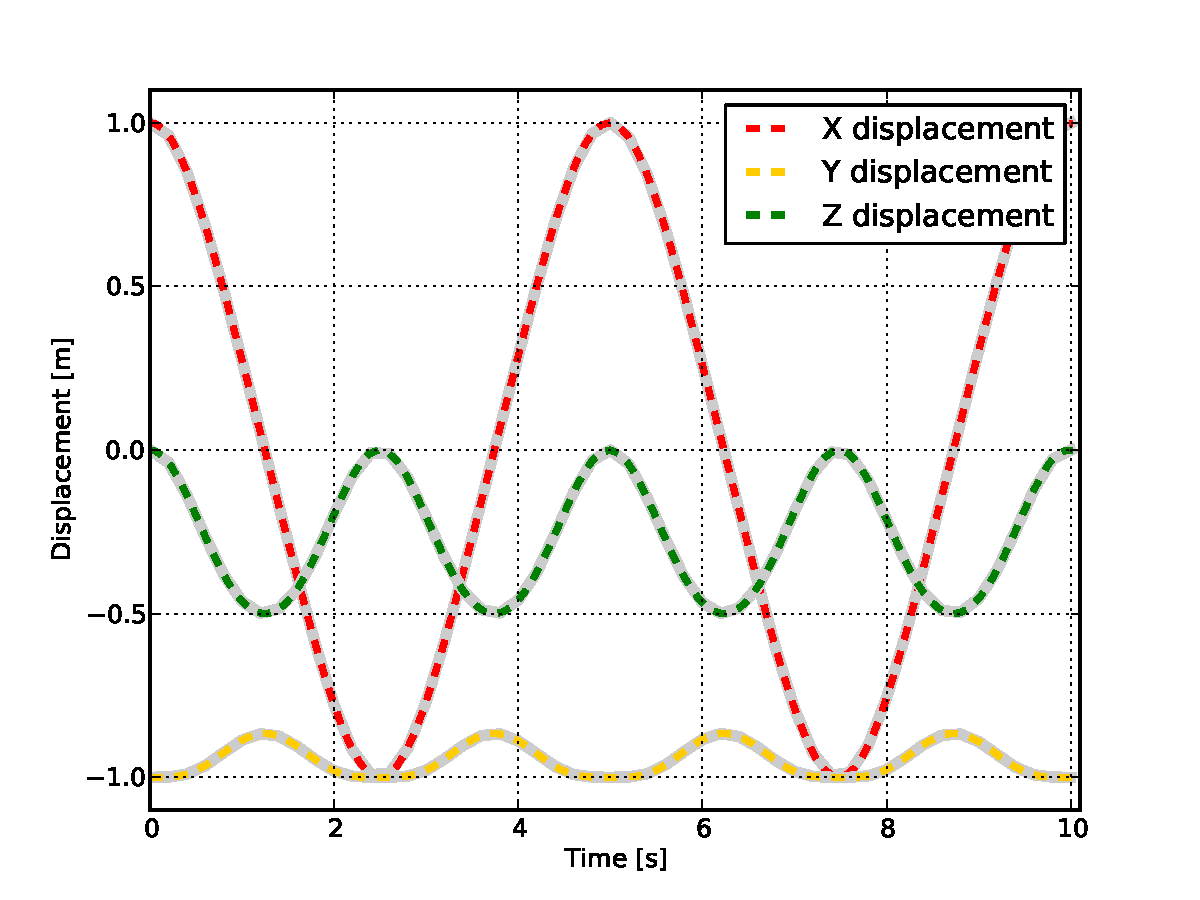
\includegraphics[width=0.95\textwidth]{4MBS_PlotResults.pdf}
\caption{$P_3$ displacements in OpenSim simulation
(dashed lines) and MBS benchmark reference values (gray lines).}
\label{FIG:simulationPlot}
\end{figure}

\end{block}
\end{column}
  

\end{columns}


\end{column}

\begin{column}{0.95\onecolwid} % The third column
\begin{block}{Download}
\begin{itemize}
\item MBS Benchmark available at: \url{http://goo.gl/ySQ5me}
\item OpenSim implementation available at: \url{http://goo.gl/R9tl3z}
\item Videos of OpenSim simulation available at: \url{http://goo.gl/8RF6nR}
\end{itemize}
\end{block}
%----------------------------------------------------------------------------------------
%	REFERENCES
%----------------------------------------------------------------------------------------

\begin{block}{References}

\begin{thebibliography}{99}

\bibitem{bricard1897memorie} Bricard R. \textit{''M{\'e}moire sur la th{\'e}orie de l'octa{\'e}dre articul{\'e}''}, in Journal de Math{\'e}matiques pures et appliqu{\'e}es, Liouville 3, 1897, pp. 113–148. 

\bibitem{grubler1884allgemeine} M. Gr{\"u}bler, \textit{``Allgemeine Eigenschaften der zwangl{\"a}ufigen ebenen kinematischen Ketten,''} Ed. Simion, 1884.

\bibitem{gonzalez2006benchmarking} M. Gonz{\'a}lez, D. Dopico, U. Lugr{\'\i}s, J. Cuadrado, \textit{``A benchmarking system for MBS simulation software: Problem standardization and performance measurement''}, 	in Multibody System Dyn., vol. 6, no.2,  2006, pp. 179--190.

\end{thebibliography}

\end{block}
\vspace{30cm}
\setbeamercolor{block alerted title}{fg=black,bg=norange} % Change the alert block title colors
\setbeamercolor{block alerted body}{fg=black,bg=white} % Change the alert block body colors

\begin{alertblock}{Contact Information}
Rehabilitation Engineering Group\\Department of Management and Engineering\\ University of Padua

\begin{itemize}
\item Web: \href{http://reg.gest.unipd.it}{http://reg.gest.unipd.it}
\item Email: \href{mailto:reg.info@gest.unipd.it}{reg.info@gest.unipd.it}
\end{itemize}

\end{alertblock}

%----------------------------------------------------------------------------------------

\end{column} % End of the third column

\end{columns} % End of all the columns in the poster

\end{frame} % End of the enclosing frame

\end{document}
